\chapter{Verkkojen perusteet}

Monen ohjelmointitehtävän voi ratkaista tulkitsemalla
tehtävän verkko-on\-gel\-ma\-na ja käyttämällä
sopivaa verkkoalgoritmia.
Tyypillinen esimerkki verkosta on tieverkosto,
jonka rakenne muistuttaa luonnostaan verkkoa.
Joskus taas verkko kätkeytyy syvemmälle ongelmaan
ja sitä voi olla vaikeaa huomata.

Tässä kirjan osassa tutustumme verkkojen käsittelyyn
liittyviin tekniikoihin ja kisakoodauksessa
keskeisiin verkkoalgoritmeihin.
Aloitamme aiheeseen perehtymisen
käymällä läpi verkkoihin liittyviä käsitteitä
sekä erilaisia tapoja pitää verkkoa muistissa algoritmeissa.

\section{Käsitteitä}

\index{verkko}
\index{solmu}
\index{kaari}

\key{Verkko} muodostuu \key{solmuista}
ja niiden välisistä \key{kaarista}.
Merkitsemme tässä kirjassa
verkon solmujen määrää
muuttujalla $n$ ja kaarten määrää muuttujalla $m$.
Lisäksi numeroimme verkon solmut kokonaisluvuin
$1,2,\ldots,n$.

Esimerkiksi seuraavassa verkossa on 5 solmua ja 7 kaarta:

\begin{center}
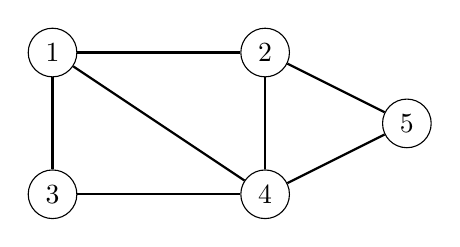
\begin{tikzpicture}[scale=0.9]
\node[draw, circle] (1) at (1,3) {$1$};
\node[draw, circle] (2) at (4,3) {$2$};
\node[draw, circle] (3) at (1,1) {$3$};
\node[draw, circle] (4) at (4,1) {$4$};
\node[draw, circle] (5) at (6,2) {$5$};

\path[draw,thick,-] (1) -- (2);
\path[draw,thick,-] (1) -- (3);
\path[draw,thick,-] (1) -- (4);
\path[draw,thick,-] (3) -- (4);
\path[draw,thick,-] (2) -- (4);
\path[draw,thick,-] (2) -- (5);
\path[draw,thick,-] (4) -- (5);
\end{tikzpicture}
\end{center}

\index{polku}

\key{Polku} on solmusta $a$ solmuun $b$
johtava reitti, joka kulkee verkon kaaria pitkin.
Polun \key{pituus} on kaarten määrä polulla.
Esimerkiksi yllä olevassa verkossa
polkuja solmusta 1 solmuun 5 ovat:

\begin{itemize}
\item $1 \rightarrow 2 \rightarrow 5$ (pituus 2)
\item $1 \rightarrow 4 \rightarrow 5$ (pituus 2)
\item $1 \rightarrow 2 \rightarrow 4 \rightarrow 5$ (pituus 3)
\item $1 \rightarrow 3 \rightarrow 4 \rightarrow 5$ (pituus 3)
\item $1 \rightarrow 3 \rightarrow 4 \rightarrow 2 \rightarrow 5$ (pituus 4)
\end{itemize}

\subsubsection{Yhtenäisyys}

\index{yhtenäinen verkko}

Verkko on \key{yhtenäinen}, jos siinä on polku
mistä tahansa solmusta mihin tahansa solmuun.
Esimerkiksi seuraava verkko on yhtenäinen:
\begin{center}
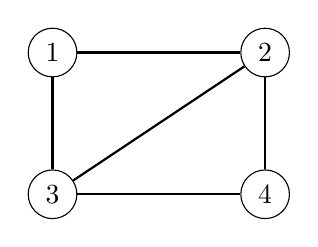
\begin{tikzpicture}[scale=0.9]
\node[draw, circle] (1) at (1,3) {$1$};
\node[draw, circle] (2) at (4,3) {$2$};
\node[draw, circle] (3) at (1,1) {$3$};
\node[draw, circle] (4) at (4,1) {$4$};
\path[draw,thick,-] (1) -- (2);
\path[draw,thick,-] (1) -- (3);
\path[draw,thick,-] (2) -- (3);
\path[draw,thick,-] (3) -- (4);
\path[draw,thick,-] (2) -- (4);
\end{tikzpicture}
\end{center}

Seuraava verkko taas ei ole yhtenäinen,
koska esimerkiksi solmusta 1 ei ole polkua solmuun 2.
\begin{center}
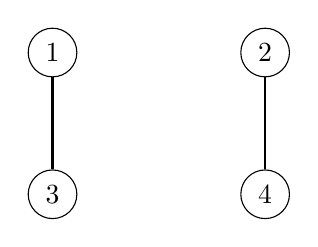
\begin{tikzpicture}[scale=0.9]
\node[draw, circle] (1) at (1,3) {$1$};
\node[draw, circle] (2) at (4,3) {$2$};
\node[draw, circle] (3) at (1,1) {$3$};
\node[draw, circle] (4) at (4,1) {$4$};
%\path[draw,thick,-] (1) -- (2);
\path[draw,thick,-] (1) -- (3);
%\path[draw,thick,-] (2) -- (3);
%\path[draw,thick,-] (3) -- (4);
\path[draw,thick,-] (2) -- (4);
\end{tikzpicture}
\end{center}

Verkon yhtenäiset osat muodostavat sen
komponentit (\textit{components}).
Esimerkiksi seuraavassa verkossa on
kolme komponenttia:
$\{1,\,2,\,3\}$,
$\{4,\,5,\,6,\,7\}$ ja
$\{8\}$.
\begin{center}
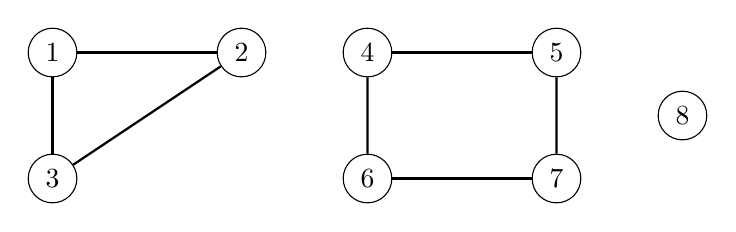
\begin{tikzpicture}[scale=0.8]
\node[draw, circle] (1) at (1,3) {$1$};
\node[draw, circle] (2) at (4,3) {$2$};
\node[draw, circle] (3) at (1,1) {$3$};

\node[draw, circle] (6) at (6,1) {$6$};
\node[draw, circle] (7) at (9,1) {$7$};
\node[draw, circle] (4) at (6,3) {$4$};
\node[draw, circle] (5) at (9,3) {$5$};

\node[draw, circle] (8) at (11,2) {$8$};

\path[draw,thick,-] (1) -- (2);
\path[draw,thick,-] (2) -- (3);
\path[draw,thick,-] (1) -- (3);
\path[draw,thick,-] (4) -- (5);
\path[draw,thick,-] (5) -- (7);
\path[draw,thick,-] (6) -- (7);
\path[draw,thick,-] (6) -- (4);
\end{tikzpicture}
\end{center}

\index{puu}

\key{Puu} on yhtenäinen verkko,
jossa on $n$ solmua ja $n-1$ kaarta.
Siinä minkä tahansa kahden solmun välillä
on yksikäsitteinen polku.
Esimerkiksi seuraava verkko on puu:

\begin{center}
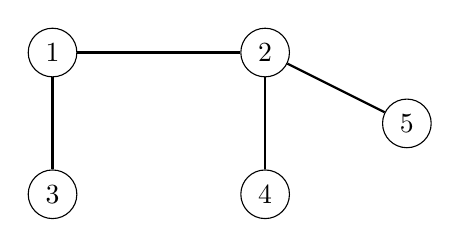
\begin{tikzpicture}[scale=0.9]
\node[draw, circle] (1) at (1,3) {$1$};
\node[draw, circle] (2) at (4,3) {$2$};
\node[draw, circle] (3) at (1,1) {$3$};
\node[draw, circle] (4) at (4,1) {$4$};
\node[draw, circle] (5) at (6,2) {$5$};

\path[draw,thick,-] (1) -- (2);
\path[draw,thick,-] (1) -- (3);
%\path[draw,thick,-] (1) -- (4);
\path[draw,thick,-] (2) -- (5);
\path[draw,thick,-] (2) -- (4);
%\path[draw,thick,-] (4) -- (5);
\end{tikzpicture}
\end{center}

\subsubsection{Kaarten suunnat}

\index{suunnattu verkko}

Verkko on \key{suunnattu},
jos verkon kaaria pystyy
kulkemaan vain niiden merkittyyn suuntaan.
Esimerkiki seuraava verkko on suunnattu:
\begin{center}
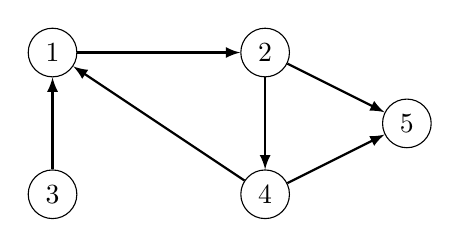
\begin{tikzpicture}[scale=0.9]
\node[draw, circle] (1) at (1,3) {$1$};
\node[draw, circle] (2) at (4,3) {$2$};
\node[draw, circle] (3) at (1,1) {$3$};
\node[draw, circle] (4) at (4,1) {$4$};
\node[draw, circle] (5) at (6,2) {$5$};
\path[draw,thick,->,>=latex] (1) -- (2);
\path[draw,thick,->,>=latex] (2) -- (4);
\path[draw,thick,->,>=latex] (2) -- (5);
\path[draw,thick,->,>=latex] (4) -- (5);
\path[draw,thick,->,>=latex] (4) -- (1);
\path[draw,thick,->,>=latex] (3) -- (1);
\end{tikzpicture}
\end{center}

Yllä olevassa verkossa solmusta 3 on polku
kaikkiin muihin verkon solmuihin.
Esimerkiksi solmusta 3 pääsee solmuun 5 pääsee polkua
$3 \rightarrow 1 \rightarrow 2 \rightarrow 5$.
Sen sijaan solmusta 5 ei lähde polkua mihinkään muuhun
solmuun.

\index{vahvasti yhtenäinen verkko}

Suunnattu verkko on \key{vahvasti yhtenäinen},
jos mistä tahansa solmusta on polku mihin
tahansa toiseen solmuun.

\index{sykli}

\key{Sykli} on polku, jonka ensimmäinen
ja viimeinen solmu on sama.
Esimerkiksi yllä olevassa verkossa on sykli
$1 \rightarrow 2 \rightarrow 4 \rightarrow 1$.
Jos verkossa ei ole yhtään sykliä, se on syklitön
(\textit{acyclic}).

\subsubsection{Kaarten painot}

\index{painotettu verkko}

\key{Painotetussa} verkossa
jokaiseen kaareen liittyy paino.
Tavallinen tulkinta on, että painot kuvaavat
kaarien pituuksia.
Seuraavassa on esimerkki painotetusta verkosta:
\begin{center}
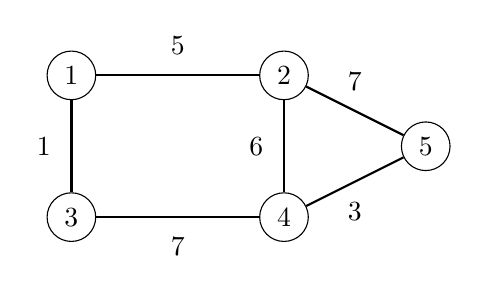
\begin{tikzpicture}[scale=0.9]
\node[draw, circle] (1) at (1,3) {$1$};
\node[draw, circle] (2) at (4,3) {$2$};
\node[draw, circle] (3) at (1,1) {$3$};
\node[draw, circle] (4) at (4,1) {$4$};
\node[draw, circle] (5) at (6,2) {$5$};
\path[draw,thick,-] (1) -- node[font=\small,label=above:5] {} (2);
\path[draw,thick,-] (1) -- node[font=\small,label=left:1] {} (3);
\path[draw,thick,-] (3) -- node[font=\small,label=below:7] {} (4);
\path[draw,thick,-] (2) -- node[font=\small,label=left:6] {} (4);
\path[draw,thick,-] (2) -- node[font=\small,label=above:7] {} (5);
\path[draw,thick,-] (4) -- node[font=\small,label=below:3] {} (5);
\end{tikzpicture}
\end{center}

Painotetussa verkossa polun pituus on sen kaarten painojen summa.
Esimerkiksi polun $1 \rightarrow 2 \rightarrow 5$
pituus on $5+7=12$ ja polun
$1 \rightarrow 3 \rightarrow 4 \rightarrow 5$ pituus on $1+7+3=11$.
Jälkimmäinen polku on lyhin polku solmusta 1 solmuun 5.

\subsubsection{Naapurit ja asteet}

\index{naapuri}
\index{aste}

Kaksi solmua ovat \key{naapureita},
jos ne ovat vierekkäin eli niiden välillä on kaari.
Solmun \key{aste} on
sen naapurien määrä.
Esimerkiksi seuraavassa verkossa
solmun 2 naapurit ovat 1, 4 ja 5,
joten sen aste on 3.

\begin{center}
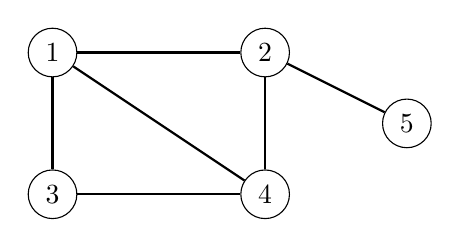
\begin{tikzpicture}[scale=0.9]
\node[draw, circle] (1) at (1,3) {$1$};
\node[draw, circle] (2) at (4,3) {$2$};
\node[draw, circle] (3) at (1,1) {$3$};
\node[draw, circle] (4) at (4,1) {$4$};
\node[draw, circle] (5) at (6,2) {$5$};

\path[draw,thick,-] (1) -- (2);
\path[draw,thick,-] (1) -- (3);
\path[draw,thick,-] (1) -- (4);
\path[draw,thick,-] (3) -- (4);
\path[draw,thick,-] (2) -- (4);
\path[draw,thick,-] (2) -- (5);
%\path[draw,thick,-] (4) -- (5);
\end{tikzpicture}
\end{center}

Verkon solmujen asteiden summa on $2m$,
missä $m$ on kaarten määrä.
Tämä johtuu siitä, että jokainen kaari lisää
kahden solmun astetta yhdellä.
Niinpä solmujen asteiden summa on aina parillinen.

\index{säännöllinen verkko}
\index{täydellinen verkko}

Verkko on \key{säännöllinen},
jos jokaisen solmun aste on vakio $d$.
Verkko on \key{täydellinen},
jos jokaisen solmun aste on $n-1$ eli
verkossa on kaikki mahdolliset kaaret
solmujen välillä.

\index{lähtöaste}
\index{tuloaste}

Suunnatussa verkossa \key{lähtöaste}
on solmusta lähtevien kaarten määrä ja
\key{tuloaste} on solmuun tulevien
kaarten määrä.
Esimerkiksi seuraavassa verkossa solmun 2
lähtöaste on 1 ja tuloaste on 2.

\begin{center}
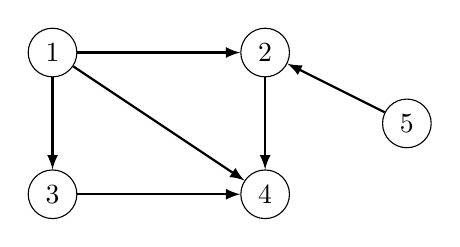
\begin{tikzpicture}[scale=0.9]
\node[draw, circle] (1) at (1,3) {$1$};
\node[draw, circle] (2) at (4,3) {$2$};
\node[draw, circle] (3) at (1,1) {$3$};
\node[draw, circle] (4) at (4,1) {$4$};
\node[draw, circle] (5) at (6,2) {$5$};

\path[draw,thick,->,>=latex] (1) -- (2);
\path[draw,thick,->,>=latex] (1) -- (3);
\path[draw,thick,->,>=latex] (1) -- (4);
\path[draw,thick,->,>=latex] (3) -- (4);
\path[draw,thick,->,>=latex] (2) -- (4);
\path[draw,thick,<-,>=latex] (2) -- (5);
\end{tikzpicture}
\end{center}

\subsubsection{Väritykset}

\index{väritys}
\index{kaksijakoinen verkko}

Verkon \key{värityksessä} jokaiselle solmulle valitaan
tietty väri niin, että millään kahdella
vierekkäisellä solmulla ei ole samaa väriä.
Verkko on \key{kaksijakoinen},
jos kaksi väriä riittää sen värittämiseen.

Esimerkiksi verkko
\begin{center}
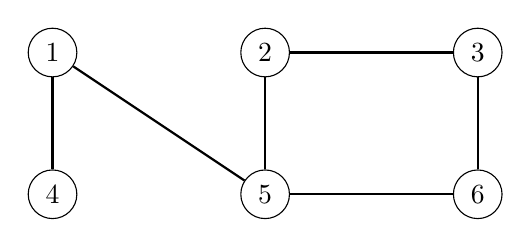
\begin{tikzpicture}[scale=0.9]
\node[draw, circle] (1) at (1,3) {$2$};
\node[draw, circle] (2) at (4,3) {$3$};
\node[draw, circle] (3) at (1,1) {$5$};
\node[draw, circle] (4) at (4,1) {$6$};
\node[draw, circle] (5) at (-2,1) {$4$};
\node[draw, circle] (6) at (-2,3) {$1$};
\path[draw,thick,-] (1) -- (2);
\path[draw,thick,-] (1) -- (3);
\path[draw,thick,-] (3) -- (4);
\path[draw,thick,-] (2) -- (4);
\path[draw,thick,-] (3) -- (6);
\path[draw,thick,-] (5) -- (6);
\end{tikzpicture}
\end{center}
on kaksijakoinen, koska sen voi värittää näin:
\begin{center}
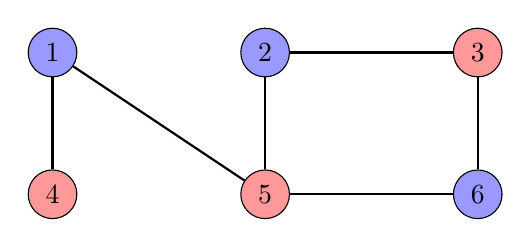
\begin{tikzpicture}[scale=0.9]
\node[draw, circle, fill=blue!40] (1) at (1,3) {$2$};
\node[draw, circle, fill=red!40] (2) at (4,3) {$3$};
\node[draw, circle, fill=red!40] (3) at (1,1) {$5$};
\node[draw, circle, fill=blue!40] (4) at (4,1) {$6$};
\node[draw, circle, fill=red!40] (5) at (-2,1) {$4$};
\node[draw, circle, fill=blue!40] (6) at (-2,3) {$1$};
\path[draw,thick,-] (1) -- (2);
\path[draw,thick,-] (1) -- (3);
\path[draw,thick,-] (3) -- (4);
\path[draw,thick,-] (2) -- (4);
\path[draw,thick,-] (3) -- (6);
\path[draw,thick,-] (5) -- (6);
\end{tikzpicture}
\end{center}

Osoittautuu, että
verkko on kaksijakoinen tarkalleen silloin,
kun siinä ei ole sykliä, johon kuuluu
pariton määrä solmuja.

\subsubsection{Yksinkertaisuus}

\index{yksinkertainen verkko}

Verkko on \key{yksinkertainen},
jos mistään solmusta ei ole kaarta itseensä
eikä minkään kahden solmun välillä ole
monta kaarta samaan suuntaan.
Usein oletuksena on, että verkko on yksinkertainen.

Esimerkiksi verkko
\begin{center}
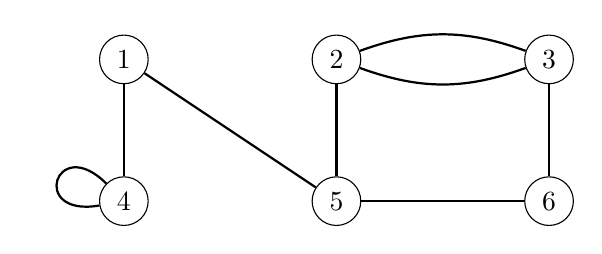
\begin{tikzpicture}[scale=0.9]
\node[draw, circle] (1) at (1,3) {$2$};
\node[draw, circle] (2) at (4,3) {$3$};
\node[draw, circle] (3) at (1,1) {$5$};
\node[draw, circle] (4) at (4,1) {$6$};
\node[draw, circle] (5) at (-2,1) {$4$};
\node[draw, circle] (6) at (-2,3) {$1$};

\path[draw,thick,-] (1) edge [bend right=20] (2);
\path[draw,thick,-] (2) edge [bend right=20] (1);
%\path[draw,thick,-] (1) -- (2);
\path[draw,thick,-] (1) -- (3);
\path[draw,thick,-] (3) -- (4);
\path[draw,thick,-] (2) -- (4);
\path[draw,thick,-] (3) -- (6);
\path[draw,thick,-] (5) -- (6);

\tikzset{every loop/.style={in=135,out=190}}
\path[draw,thick,-] (5) edge [loop left] (5);
\end{tikzpicture}
\end{center}
ei ole yksinkertainen, koska solmusta 4 on kaari itseensä
ja solmujen 2 ja 3 välillä on kaksi kaarta.

\section{Verkko muistissa}

On monia tapoja pitää verkkoa muistissa algoritmissa.
Sopiva tietorakenne riippuu siitä,
kuinka suuri verkko on ja
millä tavoin algoritmi käsittelee sitä.
Seuraavaksi käymme läpi kolme tavallista vaihtoehtoa.

\subsubsection{Vieruslistat}

\index{vieruslista}

Tavallisin tapa pitää verkkoa muistissa on
luoda jokaisesta solmusta \key{vieruslista},
joka sisältää kaikki solmut,
joihin solmusta pystyy siirtymään kaarta pitkin.
Vieruslistaesitys on tavallisin verkon esitysmuoto ja
useimmat algoritmit pystyy toteuttamaan
tehokkaasti sitä käyttäen.

Kätevä tapa tallentaa verkon vieruslistaesitys on luoda taulukko,
jossa jokainen alkio on vektori:

\begin{lstlisting}
vector<int> v[N];
\end{lstlisting}

Ideana on, että solmun $s$ vieruslista löytyy kohdasta $\texttt{v}[s]$.
Vakio $N$ on valittu niin suureksi, että kaikki solmut
mahtuvat taulukkoon.
Esimerkiksi verkon

\begin{center}
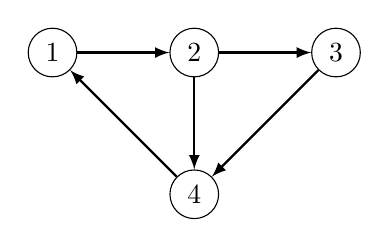
\begin{tikzpicture}[scale=0.9]
\node[draw, circle] (1) at (1,3) {$1$};
\node[draw, circle] (2) at (3,3) {$2$};
\node[draw, circle] (3) at (5,3) {$3$};
\node[draw, circle] (4) at (3,1) {$4$};

\path[draw,thick,->,>=latex] (1) -- (2);
\path[draw,thick,->,>=latex] (2) -- (3);
\path[draw,thick,->,>=latex] (2) -- (4);
\path[draw,thick,->,>=latex] (3) -- (4);
\path[draw,thick,->,>=latex] (4) -- (1);
\end{tikzpicture}
\end{center}

voi tallentaa seuraavasti:
\begin{lstlisting}
v[1].push_back(2);
v[2].push_back(3);
v[2].push_back(4);
v[3].push_back(4);
v[4].push_back(1);
\end{lstlisting}

Jos verkko on suuntaamaton, sen voi tallentaa samalla tavalla,
mutta silloin jokainen kaari lisätään kumpaankin suuntaan.

Painotetun verkon tapauksessa rakennetta voi laajentaa näin:

\begin{lstlisting}
vector<pair<int,int>> v[N];
\end{lstlisting}

Nyt vieruslistalla on pareja, joiden ensimmäinen jäsen on
kaaren kohdesolmu ja toinen jäsen on kaaren paino.
Esimerkiksi verkon

\begin{center}
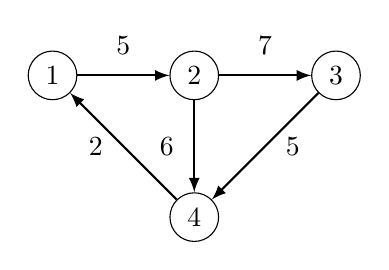
\begin{tikzpicture}[scale=0.9]
\node[draw, circle] (1) at (1,3) {$1$};
\node[draw, circle] (2) at (3,3) {$2$};
\node[draw, circle] (3) at (5,3) {$3$};
\node[draw, circle] (4) at (3,1) {$4$};

\path[draw,thick,->,>=latex] (1) -- node[font=\small,label=above:5] {} (2);
\path[draw,thick,->,>=latex] (2) -- node[font=\small,label=above:7] {} (3);
\path[draw,thick,->,>=latex] (2) -- node[font=\small,label=left:6] {} (4);
\path[draw,thick,->,>=latex] (3) -- node[font=\small,label=right:5] {} (4);
\path[draw,thick,->,>=latex] (4) -- node[font=\small,label=left:2] {} (1);
\end{tikzpicture}
\end{center}

voi tallentaa seuraavasti:
\begin{lstlisting}
v[1].push_back({2,5});
v[2].push_back({3,7});
v[2].push_back({4,6});
v[3].push_back({4,5});
v[4].push_back({1,2});
\end{lstlisting}

Vieruslistaesityksen etuna on, että sen avulla on nopeaa selvittää,
mihin solmuihin tietystä solmusta pääsee kulkemaan.
Esimerkiksi seuraava silmukka käy läpi kaikki solmut,
joihin pääsee solmusta $s$:

\begin{lstlisting}
for (auto u : v[s]) {
    // käsittele solmu u
}
\end{lstlisting}

\subsubsection{Vierusmatriisi}

\index{vierusmatriisi}

\key{Vierusmatriisi} on kaksiulotteinen taulukko,
joka kertoo jokaisesta mahdollisesta kaaresta,
onko se mukana verkossa.
Vierusmatriisista on nopeaa tarkistaa,
onko kahden solmun välillä kaari.
Toisaalta matriisi vie paljon tilaa,
jos verkko on suuri.

Vierusmatriisi tallennetaan taulukkona

\begin{lstlisting}
int v[N][N];
\end{lstlisting}

jossa arvo $\texttt{v}[a][b]$ ilmaisee,
onko kaari solmusta $a$ solmuun $b$ mukana verkossa.
Yksinkertaisin tapa luoda vierusmatriisi
on käyttää arvoja 1 (mukana) ja 0 (ei mukana).
Tällöin esimerkiksi verkkoa

\begin{center}
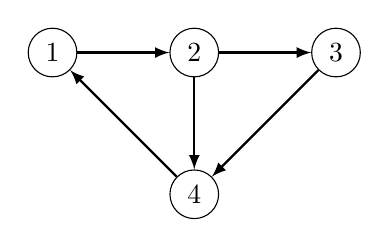
\begin{tikzpicture}[scale=0.9]
\node[draw, circle] (1) at (1,3) {$1$};
\node[draw, circle] (2) at (3,3) {$2$};
\node[draw, circle] (3) at (5,3) {$3$};
\node[draw, circle] (4) at (3,1) {$4$};

\path[draw,thick,->,>=latex] (1) -- (2);
\path[draw,thick,->,>=latex] (2) -- (3);
\path[draw,thick,->,>=latex] (2) -- (4);
\path[draw,thick,->,>=latex] (3) -- (4);
\path[draw,thick,->,>=latex] (4) -- (1);
\end{tikzpicture}
\end{center}

vastaa seuraava vierusmatriisi:

\begin{center}
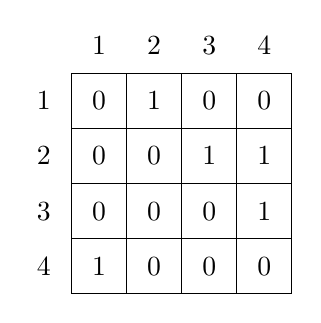
\begin{tikzpicture}[scale=0.7]
\draw (0,0) grid (4,4);
\node at (0.5,0.5) {1};
\node at (1.5,0.5) {0};
\node at (2.5,0.5) {0};
\node at (3.5,0.5) {0};
\node at (0.5,1.5) {0};
\node at (1.5,1.5) {0};
\node at (2.5,1.5) {0};
\node at (3.5,1.5) {1};
\node at (0.5,2.5) {0};
\node at (1.5,2.5) {0};
\node at (2.5,2.5) {1};
\node at (3.5,2.5) {1};
\node at (0.5,3.5) {0};
\node at (1.5,3.5) {1};
\node at (2.5,3.5) {0};
\node at (3.5,3.5) {0};
\node at (-0.5,0.5) {4};
\node at (-0.5,1.5) {3};
\node at (-0.5,2.5) {2};
\node at (-0.5,3.5) {1};
\node at (0.5,4.5) {1};
\node at (1.5,4.5) {2};
\node at (2.5,4.5) {3};
\node at (3.5,4.5) {4};
\end{tikzpicture}
\end{center}

Jos verkko on painotettu, vierusmatriisiesitystä voi 
laajentaa luontevasti niin, että matriisissa kerrotaan
kaaren paino, jos kaari on olemassa.
Tätä esitystapaa käyttäen esimerkiksi verkkoa

\begin{center}
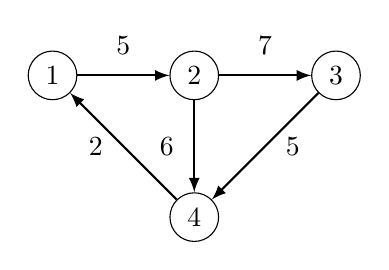
\begin{tikzpicture}[scale=0.9]
\node[draw, circle] (1) at (1,3) {$1$};
\node[draw, circle] (2) at (3,3) {$2$};
\node[draw, circle] (3) at (5,3) {$3$};
\node[draw, circle] (4) at (3,1) {$4$};

\path[draw,thick,->,>=latex] (1) -- node[font=\small,label=above:5] {} (2);
\path[draw,thick,->,>=latex] (2) -- node[font=\small,label=above:7] {} (3);
\path[draw,thick,->,>=latex] (2) -- node[font=\small,label=left:6] {} (4);
\path[draw,thick,->,>=latex] (3) -- node[font=\small,label=right:5] {} (4);
\path[draw,thick,->,>=latex] (4) -- node[font=\small,label=left:2] {} (1);
\end{tikzpicture}
\end{center}

vastaa seuraava vierusmatriisi:

\begin{center}
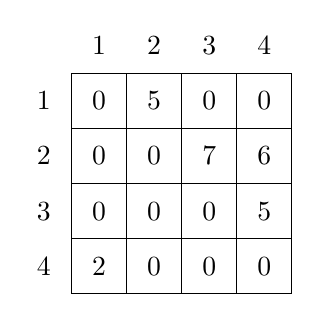
\begin{tikzpicture}[scale=0.7]
\draw (0,0) grid (4,4);
\node at (0.5,0.5) {2};
\node at (1.5,0.5) {0};
\node at (2.5,0.5) {0};
\node at (3.5,0.5) {0};
\node at (0.5,1.5) {0};
\node at (1.5,1.5) {0};
\node at (2.5,1.5) {0};
\node at (3.5,1.5) {5};
\node at (0.5,2.5) {0};
\node at (1.5,2.5) {0};
\node at (2.5,2.5) {7};
\node at (3.5,2.5) {6};
\node at (0.5,3.5) {0};
\node at (1.5,3.5) {5};
\node at (2.5,3.5) {0};
\node at (3.5,3.5) {0};
\node at (-0.5,0.5) {4};
\node at (-0.5,1.5) {3};
\node at (-0.5,2.5) {2};
\node at (-0.5,3.5) {1};
\node at (0.5,4.5) {1};
\node at (1.5,4.5) {2};
\node at (2.5,4.5) {3};
\node at (3.5,4.5) {4};
\end{tikzpicture}
\end{center}

\subsubsection{Kaarilista}

\index{kaarilista}

\key{Kaarilista} sisältää kaikki verkon kaaret.
Kaarilista on hyvä tapa tallentaa verkko,
jos algoritmissa täytyy käydä läpi
kaikki verkon kaaret eikä ole tarvetta
etsiä kaarta alkusolmun perusteella.

Kaarilistan voi tallentaa vektoriin
\begin{lstlisting}
vector<pair<int,int>> v;
\end{lstlisting}
jossa jokaisessa solmussa on parina kaaren
alku- ja loppusolmu.
Tällöin esimerkiksi verkon

\begin{center}
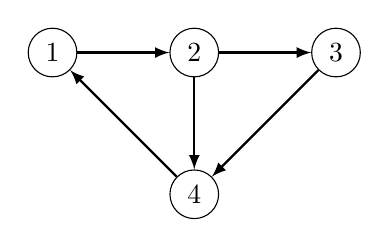
\begin{tikzpicture}[scale=0.9]
\node[draw, circle] (1) at (1,3) {$1$};
\node[draw, circle] (2) at (3,3) {$2$};
\node[draw, circle] (3) at (5,3) {$3$};
\node[draw, circle] (4) at (3,1) {$4$};

\path[draw,thick,->,>=latex] (1) -- (2);
\path[draw,thick,->,>=latex] (2) -- (3);
\path[draw,thick,->,>=latex] (2) -- (4);
\path[draw,thick,->,>=latex] (3) -- (4);
\path[draw,thick,->,>=latex] (4) -- (1);
\end{tikzpicture}
\end{center}
voi tallentaa seuraavasti:
\begin{lstlisting}
v.push_back({1,2});
v.push_back({2,3});
v.push_back({2,4});
v.push_back({3,4});
v.push_back({4,1});
\end{lstlisting}

\noindent
Painotetun verkon tapauksessa rakennetta voi laajentaa
esimerkiksi näin:
\begin{lstlisting}
vector<pair<pair<int,int>,int>> v;
\end{lstlisting}
Ideana on, että listalla on pareja, joiden ensimmäinen jäsen
sisältää parina kaaren alku- ja loppusolmun,
ja toinen jäsen on kaaren paino.
Nyt verkon

\begin{center}
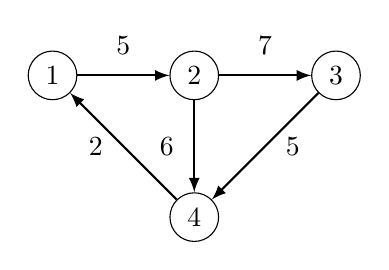
\begin{tikzpicture}[scale=0.9]
\node[draw, circle] (1) at (1,3) {$1$};
\node[draw, circle] (2) at (3,3) {$2$};
\node[draw, circle] (3) at (5,3) {$3$};
\node[draw, circle] (4) at (3,1) {$4$};

\path[draw,thick,->,>=latex] (1) -- node[font=\small,label=above:5] {} (2);
\path[draw,thick,->,>=latex] (2) -- node[font=\small,label=above:7] {} (3);
\path[draw,thick,->,>=latex] (2) -- node[font=\small,label=left:6] {} (4);
\path[draw,thick,->,>=latex] (3) -- node[font=\small,label=right:5] {} (4);
\path[draw,thick,->,>=latex] (4) -- node[font=\small,label=left:2] {} (1);
\end{tikzpicture}
\end{center}

voi tallentaa seuraavasti:

\begin{lstlisting}
v.push_back({{1,2},5});
v.push_back({{2,3},7});
v.push_back({{2,4},6});
v.push_back({{3,4},5});
v.push_back({{4,1},2});
\end{lstlisting}


